\section{Deep models detail}
\label{sec:Deep models detail}
% 7.5 pages
Machine learning is a branch of artificial intelligence. Deep learning is also a branch of machine learning, which utilises artificial neural networks for feature learning and hierarchical feature extraction to replace manual feature engineering in other machine learning methods.
Recently, the research of deep learning is a hot topic in the field of computer science, and it is also an important method used in the computer vision task in this research.
This section will introduce the details of a variety of deep learning models related to this research, including CNN, RNN, attention and Transformer structures.
Although the applications or target tasks of these models are different, the design ideas between them are mutually influential.
Therefore, reviewing the development and design concepts of these previous models will greatly help the design of the model in this research.

\subsection{Convolutional neural network} % 2.5 pages
With the rapid development of neurobiology and cognitive science, the concept of artificial neural networks, a computational model that imitates the structure and function of biological neural networks, has been proposed as early as the last century.
\citet{fukushima1980neocognitron} proposes a network created from the animal visual system as well as some key concepts, such as \textbf{local receptive field}, \textbf{multi-layer perception architecture} and translation \textbf{equivariance and invariance property} (not affected by shift in position).

In detail, the local receptive field means that each neuron will not perceive the image as a whole, it will only perceive the local information, then the local perception can be integrated through a multi-layer perception architecture to obtain the global perception.
On the other hand, the property of translation equivariance and invariance is emerging from the combination of the local receptive field and multi-layer perception architecture.

The study of neurobiology and cognitive science is then evolved into a computational model. For example, \citet{zhang1988shift} propose the first two-dimensional Shift Invariant Artificial Neural Network (SIANN).
Then, \citet{lecun1989backpropagation} propose a original CNN with two convolutional layers and two fully connected layers using backpropagation method to train in a supervised learning approach.
They also highlight the term convolution for the first time, and named this model type as convolutional neural network (CNN).
Soon after the application of this model in handwritten zip code recognition, \citet{zhang1994computerized} apply it to a practical case of recognising medical imagery.

\begin{figure}[ht!]
    \centering
    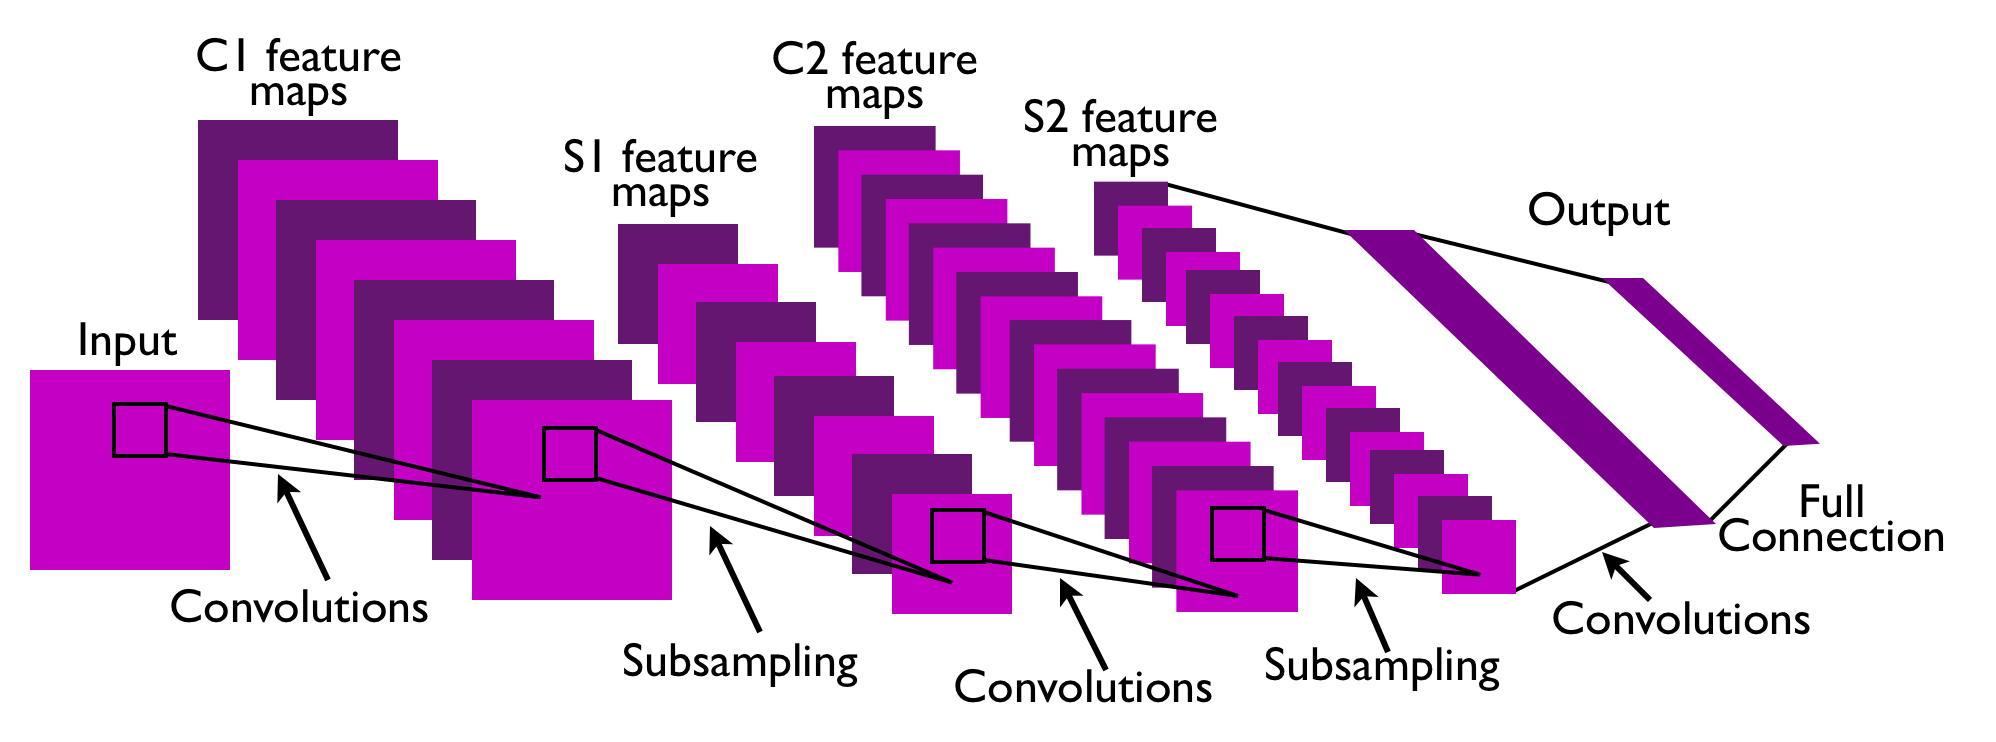
\includegraphics[width=\textwidth]{literature/imgs/ext-lecun-cnn-arch.png}
    \caption{CNN applications in vision by \citet{lecun2010convolutional}}
    \label{fig:ext-lecun-cnn-arch}
\end{figure}

The most revolutionary progress is that \citet{lecun2010convolutional} propose a modern architecture for this model, as illustrated in figure \ref{fig:ext-lecun-cnn-arch}.
This structure comprises three convolutional layers combined in between with two sub-sampling layers, and two fully connected layers. Sub-sampling, also known as pooling, reduces the size of feature maps, by retaining only important information to simplify calculation.
Further, it further strengthens the translation invariance, taking maximum pooling as example, because the translation does not affect the maximum value, the pooling result remains unchanged.

In the following years of development of CNN, the number of layers in deep networks is gradually deepening to obtain greater high-level information.
In 2012, \citet{krizhevsky2012imagenet} propose AlexNet which use 5 convolutional layers and 3 fully connected layers.
However, as the number of hidden layers increases, the model gets more complex and prone to overfitting.
AlexNet uses the Dropout layer by randomly breaking neuron connection (setting random input units to zero) in training process to prevent overfitting. 
Two years later, \citet{simonyan2014very} propose Visual Geometry Group (VGG) model, in which $3\times3$ size convolution kernels are fully used in a total of 5 layers, just as the title of the paper, it is a very deep convolutional network.

The experiment in the VGG model concludes that the deeper the number of network layers, the better the performance.
However, as the depth of the model and the number of parameters continue to increase, the following two significant problems have been discovered.

\begin{enumerate}
    \item The network is prone to overfit, requiring more training data, making it more difficult to train.
    \item More storage resources and computing resources are required, but cannot provide adequate performance boost. 
\end{enumerate}

In order to solve these problems, \citet{he2015deep} propose a residual structure to make deep network training easier with enhanced performance but fewer parameters and lower complexity. 
They first identify that the root cause of these problems is that the deeper network structure leads to degradation, i.e., the training error and the verification error both increase since the deeper network does not learn anything but loses useful features.
Then, figure \ref{fig:ext-CNN-ResNet-BBs} illustrates two types of building blocks used in ResNets with different number of layers.
The first typical block just uses cross-layer connection, a linear layer from input to output connected directly.
By denoting the desired underlying mapping as $H(x)$, the each layer learns the residual between input $x$ and desired output $F(x):=H(x)-x$.
As a result, such a residual structure allows the deep network to adapt to the appropriate depth, i.e., use the identity transform across unnecessary layers.

Further, figure \ref{fig:ext-CNN-ResNet} compares the network structure of VGG-19, 34-layer plain, and 34-layer residual and shows how to use the building block in the actual deep network. Figure \ref{fig:ext-CNN-ResNet-BBs} also shows a ``bottleneck'' building block for deeper ResNets, which first uses a $1\times1$ size convolution to reduce the dimensional across channels to reduce the calculation required in the $3\times3$ convolution.

\begin{minipage}[ht]{.32\textwidth}
    \begin{figure}[H]
        \centering
    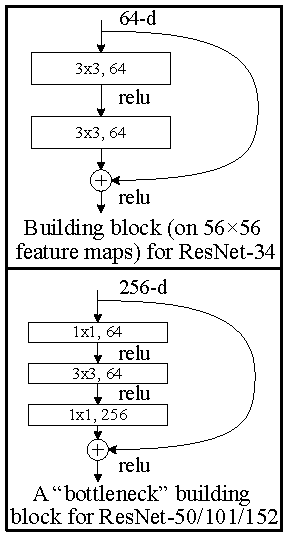
\includegraphics[width=.99\textwidth]{literature/imgs/ext-CNN-ResNet-BBs.pdf}
    \caption{Residual building blocks by \citet{he2015deep}}
    \label{fig:ext-CNN-ResNet-BBs}
    \end{figure}
\end{minipage}
\hspace{1em}
\begin{minipage}[ht]{.62\textwidth}
    \begin{figure}[H]
        \centering
    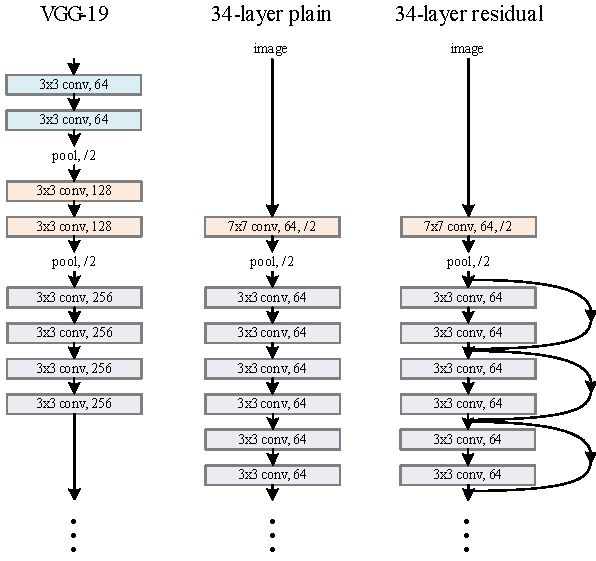
\includegraphics[width=.99\textwidth]{literature/imgs/ext-CNN-ResNet.pdf}
    \caption{VGG and Residual ImageNet by \citet{he2015deep}}
    \label{fig:ext-CNN-ResNet}
    \end{figure}
\end{minipage}

\subsection{Recurrent neural network} % 2.5 pages
\citet{jordan1997serial}

%LSTM
\citet{hochreiter1997long}

% RNN & LSTM fundamentals summary
\citet{sherstinsky2020fundamentals}

%GRU
\citet{chung2014empirical}

Sequential computing restriction and long-term memory loss issues.

\subsection{Attention and Transformer} % 2.5 pages
%Attention
\citet{bahdanau2016neural}

\begin{minipage}[ht]{.6\textwidth}
    \begin{figure}[H]
        \centering
        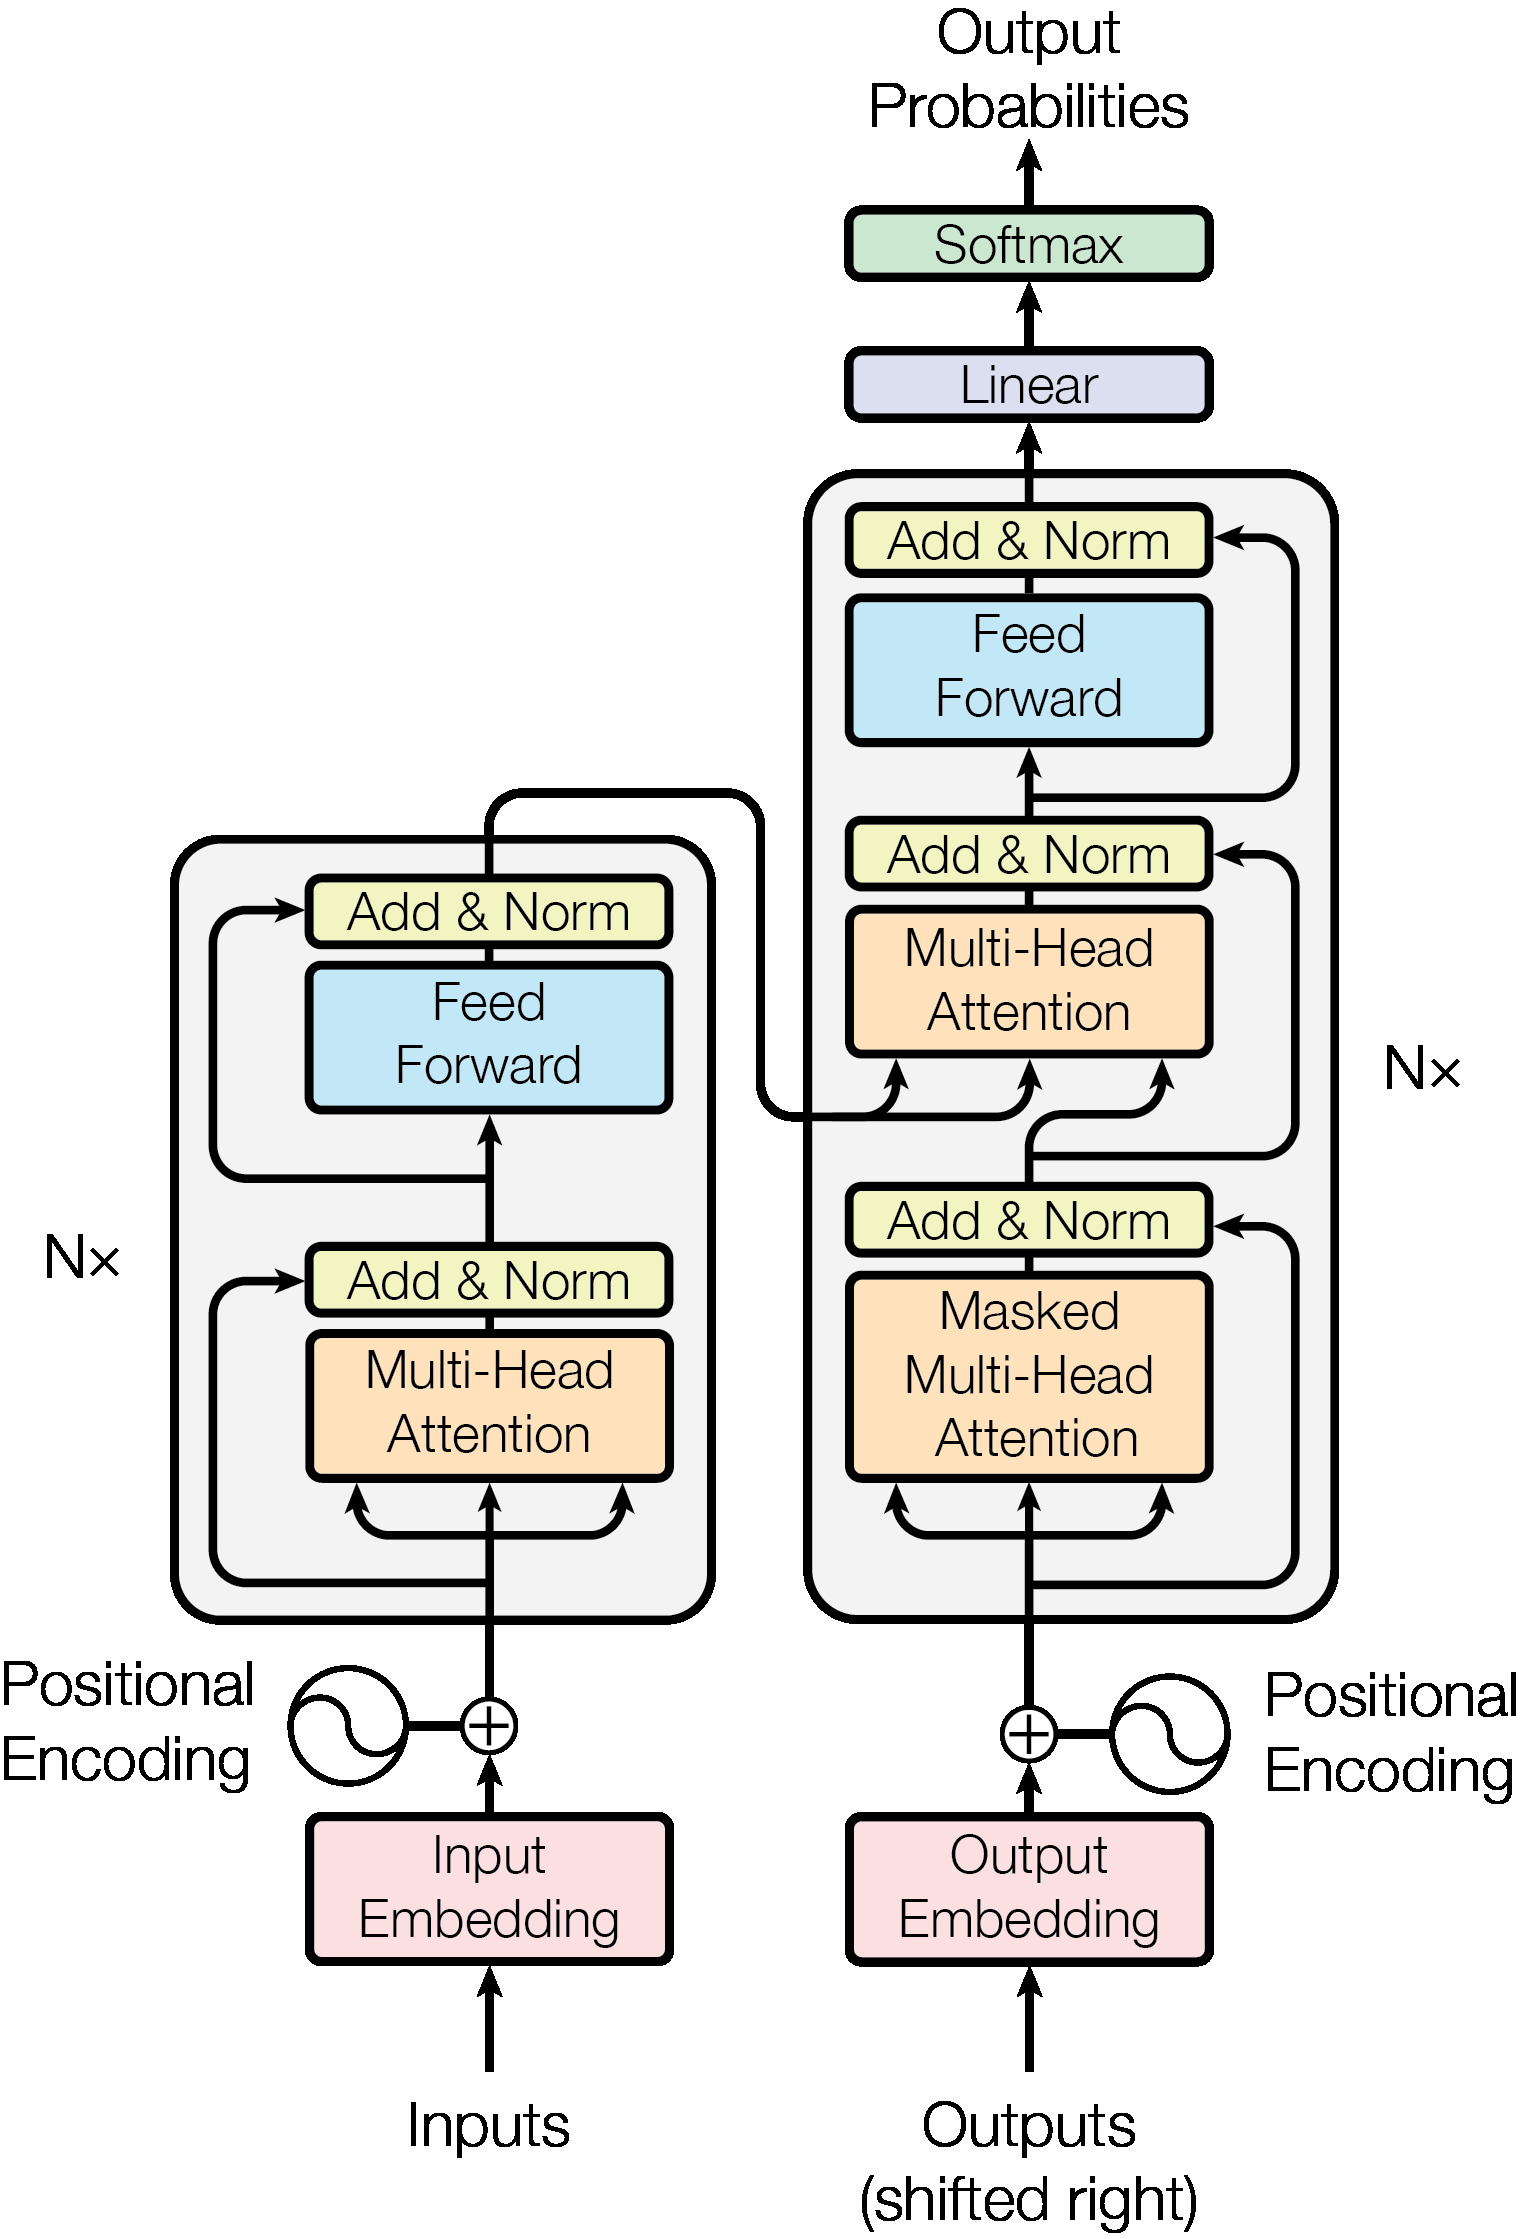
\includegraphics[width=\textwidth]{literature/imgs/ext-transformer.png}
        \caption{The Transformer model architecture \cite{vaswani2017attention}}
        \label{fig:ext-transformer}
    \end{figure}
\end{minipage}
\begin{minipage}[ht]{.35\textwidth}
    \centering
    \begin{figure}[H]
        \centering
        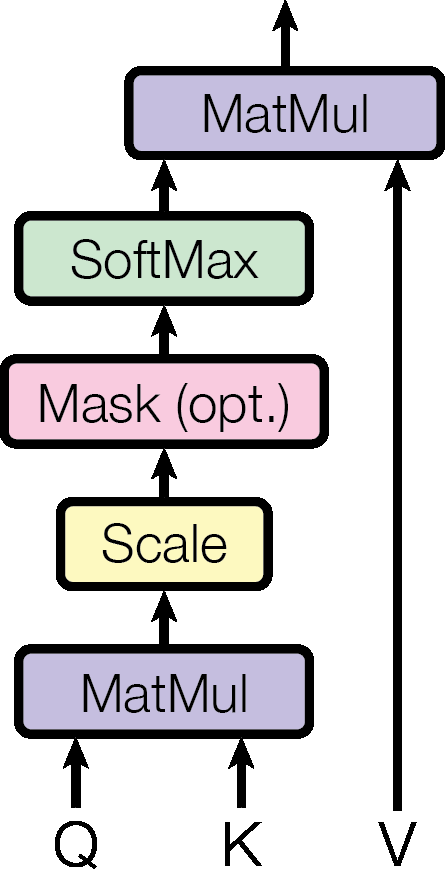
\includegraphics[width=.48\textwidth]{literature/imgs/ext-attention-dot-product.png}
        \caption{Scaled Dot-Product Attention \cite{vaswani2017attention}}
        \label{fig:ext-attention-dot-product}
    \end{figure}
    \vspace*{-.5cm}
    \begin{figure}[H]
        \centering
        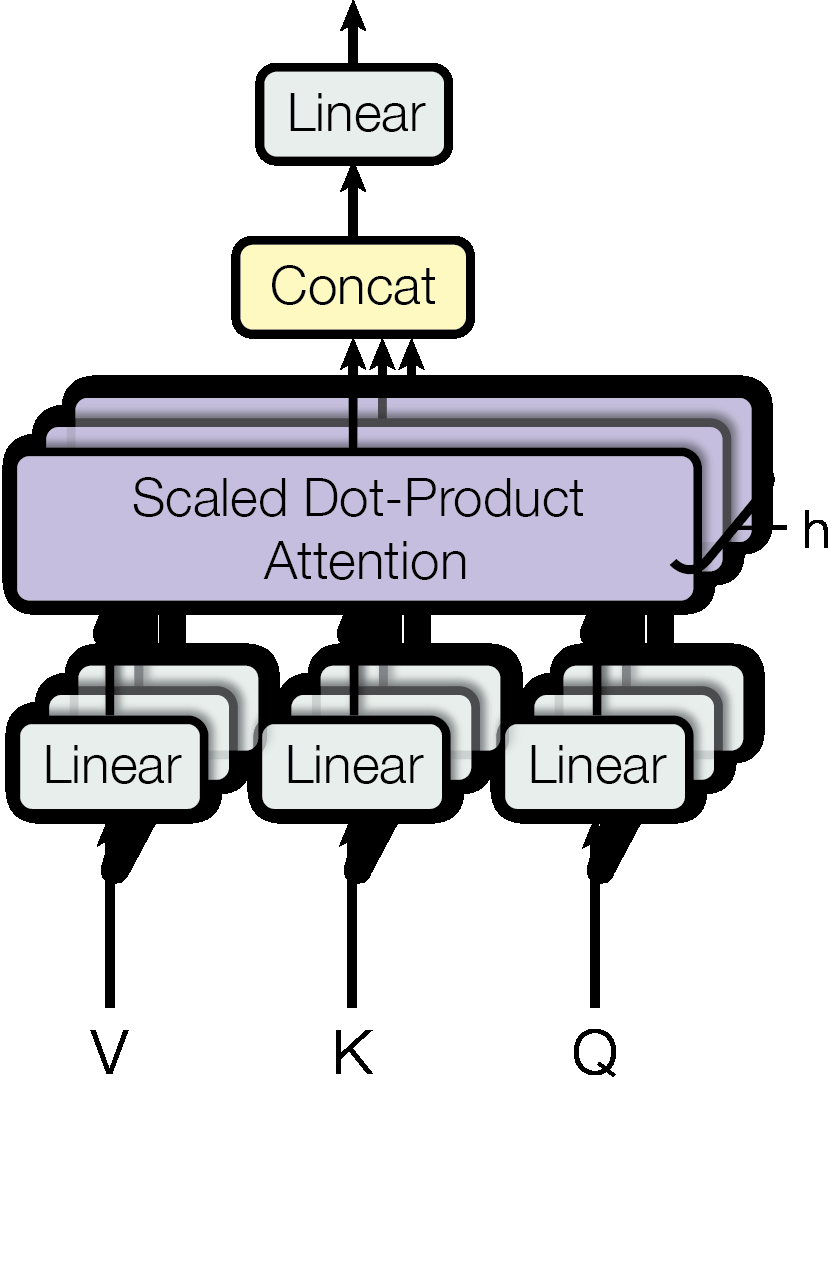
\includegraphics[width=.9\textwidth]{literature/imgs/ext-attention-multihead.png}
        \vspace*{-.4cm}
        \caption{Multi-Head Attention \cite{vaswani2017attention}}
        \label{fig:ext-attention-multihead}
    \end{figure}
\end{minipage}

\citet{vaswani2017attention}

%Transformer
While convolutional neural network (CNN) is in the ascendant among the fields of computer vision, transformer model composed of self-attention structures has achieved state-of-the-art results in many natural language processing tasks.

\citet{devlin2019bert}

The transformer model gradually replaced the recurrent neural network (RRN) with sequential computing restriction and long-term memory loss issues.

\subsection{State-of-the-art models}

Innovative design concepts from the transformer model are also carried forward in the fields of computer vision.

Many recent studies, such as Data-efficient image Transformers (DeiT) and Shifted window (Swin) transformers, have improved widely-adopted CNN-only models such as VGG and ResNet by introducing the self-attention structures to achieve better performance.

\citet{srinivas2021bottleneck}

\citet{wang2021pyramid}

\citet{dai2021coatnet}
